% latex table generated in R 3.6.3 by xtable 1.8-4 package
% Thu Jan 18 11:50:01 2024
\begin{table}[ht]
\centering
\begin{tabular}{rlrrr}
  \hline
 & OTU & MeanRA & MedianRA & SE \\ 
  \hline
2725558 & Parasphingorhabdus halotoleran & 0.00004942 & 0.00005047 & 0.00000253 \\ 
  2018065 & Roseomonas sp. FDAARGOS\_36 & 0.00006303 & 0.00006015 & 0.00000550 \\ 
  207340 & Roseomonas mucos & 0.00006631 & 0.00006188 & 0.00000593 \\ 
  265960 & Komagataeibacter nataicol & 0.00005453 & 0.00005675 & 0.00000304 \\ 
  65958 & Komagataeibacter oboedien & 0.00004356 & 0.00004265 & 0.00000366 \\ 
  1510841 & Parasaccharibacter apiu & 0.00003894 & 0.00003873 & 0.00000249 \\ 
  2587846 & Roseovarius sp. THAF & 0.00005102 & 0.00005217 & 0.00000246 \\ 
  114277 & Rickettsia & 0.00001872 & 0.00001483 & 0.00000238 \\ 
  2582913 & Luteithermobacter gelatinilyticu & 0.00006527 & 0.00006616 & 0.00000363 \\ 
  32009 & Burkholderia gladioli & 0.00004830 & 0.00004972 & 0.00000308 \\ 
  428406 & Ralstonia pickettii & 0.00003543 & 0.00003411 & 0.00000352 \\ 
  2705547 & Caballeronia sp. SBC & 0.00001283 & 0.00001306 & 0.00000171 \\ 
  521 & Bordetella aviu & 0.00007239 & 0.00007953 & 0.00000767 \\ 
  2813780 & Alcaligenes sp. SORT2 & 0.00002027 & 0.00001982 & 0.00000134 \\ 
  2735906 & Pseudomonas sp. B11D7 & 0.00007674 & 0.00006215 & 0.00001262 \\ 
  2498848 & Pseudomonas sp. MPC & 0.00005337 & 0.00005810 & 0.00000486 \\ 
  2049589 & Pseudomonas sp. HLS- & 0.00005016 & 0.00004639 & 0.00000601 \\ 
  2320270 & Pseudomonas sp. DG56- & 0.00004195 & 0.00004099 & 0.00000337 \\ 
  253237 & Pseudomonas sp. phDV & 0.00002511 & 0.00002117 & 0.00000454 \\ 
  2054915 & Pseudomonas sp. 09C 12 & 0.00001342 & 0.00000816 & 0.00000359 \\ 
  47879 & Pseudomonas corrugat & 0.00005569 & 0.00005675 & 0.00000521 \\ 
  29442 & Pseudomonas tolaasi & 0.00004202 & 0.00004401 & 0.00000331 \\ 
  86185 & Pseudomonas lundensi & 0.00004760 & 0.00004792 & 0.00000292 \\ 
  33069 & Pseudomonas viridiflav & 0.00005855 & 0.00005540 & 0.00000478 \\ 
  36746 & Pseudomonas cichori & 0.00005742 & 0.00005405 & 0.00000595 \\ 
  1301098 & Pseudomonas knackmussii & 0.00004742 & 0.00005061 & 0.00000490 \\ 
  384676 & Pseudomonas entomophila & 0.00007598 & 0.00007353 & 0.00000504 \\ 
  364197 & Pseudomonas pohangensi & 0.00007718 & 0.00007531 & 0.00000776 \\ 
  1434072 & Halopseudomonas salegen & 0.00005062 & 0.00004926 & 0.00000475 \\ 
  1274359 & Pseudomonas sihuiensi & 0.00003523 & 0.00003108 & 0.00000475 \\ 
  163011 & Pseudomonas lin & 0.00004334 & 0.00003403 & 0.00001151 \\ 
  2681387 & Klebsiella sp. STW0522-4 & 0.00000430 & 0.00000442 & 0.00000051 \\ 
  546 & Citrobacter freundi & 0.00004584 & 0.00004594 & 0.00000284 \\ 
  1300165 & Kosakonia cowanii & 0.00000466 & 0.00000315 & 0.00000096 \\ 
  551989 & Kosakonia arachidi & 0.00001129 & 0.00001178 & 0.00000096 \\ 
  2681308 & Leclercia sp. 11928 & 0.00000435 & 0.00000393 & 0.00000042 \\ 
  1972431 & Phytobacter ursingi & 0.00001194 & 0.00001270 & 0.00000123 \\ 
  1048758 & Candidatus Moranella endobi & 0.00000622 & 0.00000577 & 0.00000141 \\ 
  2033438 & Serratia sp. MYb23 & 0.00000908 & 0.00001054 & 0.00000128 \\ 
  1484158 & Pantoea sp. PSNIH & 0.00002788 & 0.00002880 & 0.00000215 \\ 
  1615494 & Mixta intestinali & 0.00002092 & 0.00002090 & 0.00000188 \\ 
  1089444 & Dickeya solan & 0.00001319 & 0.00001367 & 0.00000171 \\ 
  2609667 & Halomonas piezotoleran & 0.00003279 & 0.00003365 & 0.00000203 \\ 
  33074 & Zymobacter palma & 0.00002873 & 0.00003009 & 0.00000209 \\ 
  1921086 & Mariprofundus aestuariu & 0.00002417 & 0.00002574 & 0.00000198 \\ 
  67351 & Streptomyces californicu & 0.00005978 & 0.00006206 & 0.00000419 \\ 
  1906 & Streptomyces fradia & 0.00003934 & 0.00003811 & 0.00000365 \\ 
  285473 & Streptomyces rubrolavendula & 0.00003242 & 0.00003359 & 0.00000313 \\ 
  145458 & Rathayibacter toxicu & 0.00003871 & 0.00003751 & 0.00000311 \\ 
  2623385 & Aurantimicrobium & 0.00002175 & 0.00002223 & 0.00000089 \\ 
  1667168 & Dermabacter jinjuensi & 0.00006693 & 0.00007026 & 0.00000481 \\ 
  472569 & Devriesea agamaru & 0.00003782 & 0.00004075 & 0.00000274 \\ 
  1863 & Dermatophilus congolensi & 0.00002880 & 0.00003130 & 0.00000274 \\ 
  110539 & Mycolicibacterium vanbaaleni & 0.00004566 & 0.00004389 & 0.00000245 \\ 
  39687 & Mycolicibacterium austroafricanu & 0.00004749 & 0.00004724 & 0.00000247 \\ 
  441500 & Corynebacterium timonens & 0.00008281 & 0.00009011 & 0.00000606 \\ 
  136857 & Corynebacterium testudinori & 0.00005339 & 0.00005098 & 0.00000452 \\ 
  38288 & Corynebacterium genitaliu & 0.00004085 & 0.00004418 & 0.00000348 \\ 
  1050174 & Corynebacterium epidermidicani & 0.00002787 & 0.00003085 & 0.00000210 \\ 
  1724 & Corynebacterium renal & 0.00002763 & 0.00002957 & 0.00000201 \\ 
  84096 & Gordonia alkanivoran & 0.00003676 & 0.00003844 & 0.00000315 \\ 
  40567 & Actinosynnema miru & 0.00002690 & 0.00002796 & 0.00000256 \\ 
  1960083 & Actinomyces gaoshouyi & 0.00004936 & 0.00005059 & 0.00000374 \\ 
  1335613 & Gordonibacter urolithinfacien & 0.00008030 & 0.00009091 & 0.00000884 \\ 
  1126833 & Paenibacillus beijingensi & 0.00007284 & 0.00007434 & 0.00000373 \\ 
  1214604 & Tumebacillus algifaeci & 0.00006178 & 0.00005998 & 0.00000365 \\ 
  1584 & Lactobacillus delbruecki & 0.00002521 & 0.00002645 & 0.00000200 \\ 
  1871021 & Lachnoclostridium phocaeens & 0.00002102 & 0.00002223 & 0.00000235 \\ 
  252966 & Mahella australiensi & 0.00001838 & 0.00001963 & 0.00000242 \\ 
  2487118 & Intestinibaculum porc & 0.00000884 & 0.00000907 & 0.00000167 \\ 
  44471 & Microcoleu & 0.00002284 & 0.00002396 & 0.00000247 \\ 
  289435 & Sphaerospermopsis kisselevian & 0.00001241 & 0.00000986 & 0.00000255 \\ 
  1851148 & Limihaloglobus sulfuriphilu & 0.00003148 & 0.00003053 & 0.00000255 \\ 
  180 & Leptospirillum sp. Group I & 0.00001822 & 0.00001622 & 0.00000160 \\ 
  665571 & Spirochaeta thermophila & 0.00003221 & 0.00003433 & 0.00000277 \\ 
  693075 & Caldisericum exil & 0.00001933 & 0.00001959 & 0.00000236 \\ 
  430914 & Halorhabdus tiamate & 0.00004053 & 0.00004514 & 0.00000345 \\ 
  2226 & Methanococcoides methyluten & 0.00000386 & 0.00000405 & 0.00000067 \\ 
  2224 & Methanothrix thermoacetophil & 0.00000918 & 0.00000940 & 0.00000110 \\ 
  1470067 & Nitrosopumilus ureiphilu & 0.00000750 & 0.00000761 & 0.00000199 \\ 
  1874277 & Conexivisphaera calid & 0.00001650 & 0.00001683 & 0.00000221 \\ 
  184117 & Thermoproteus uzoniensi & 0.00001875 & 0.00002151 & 0.00000194 \\ 
   \hline
\end{tabular}
\caption{Keystone OTUs of } 
\end{table}
\begin{figure}
\centering
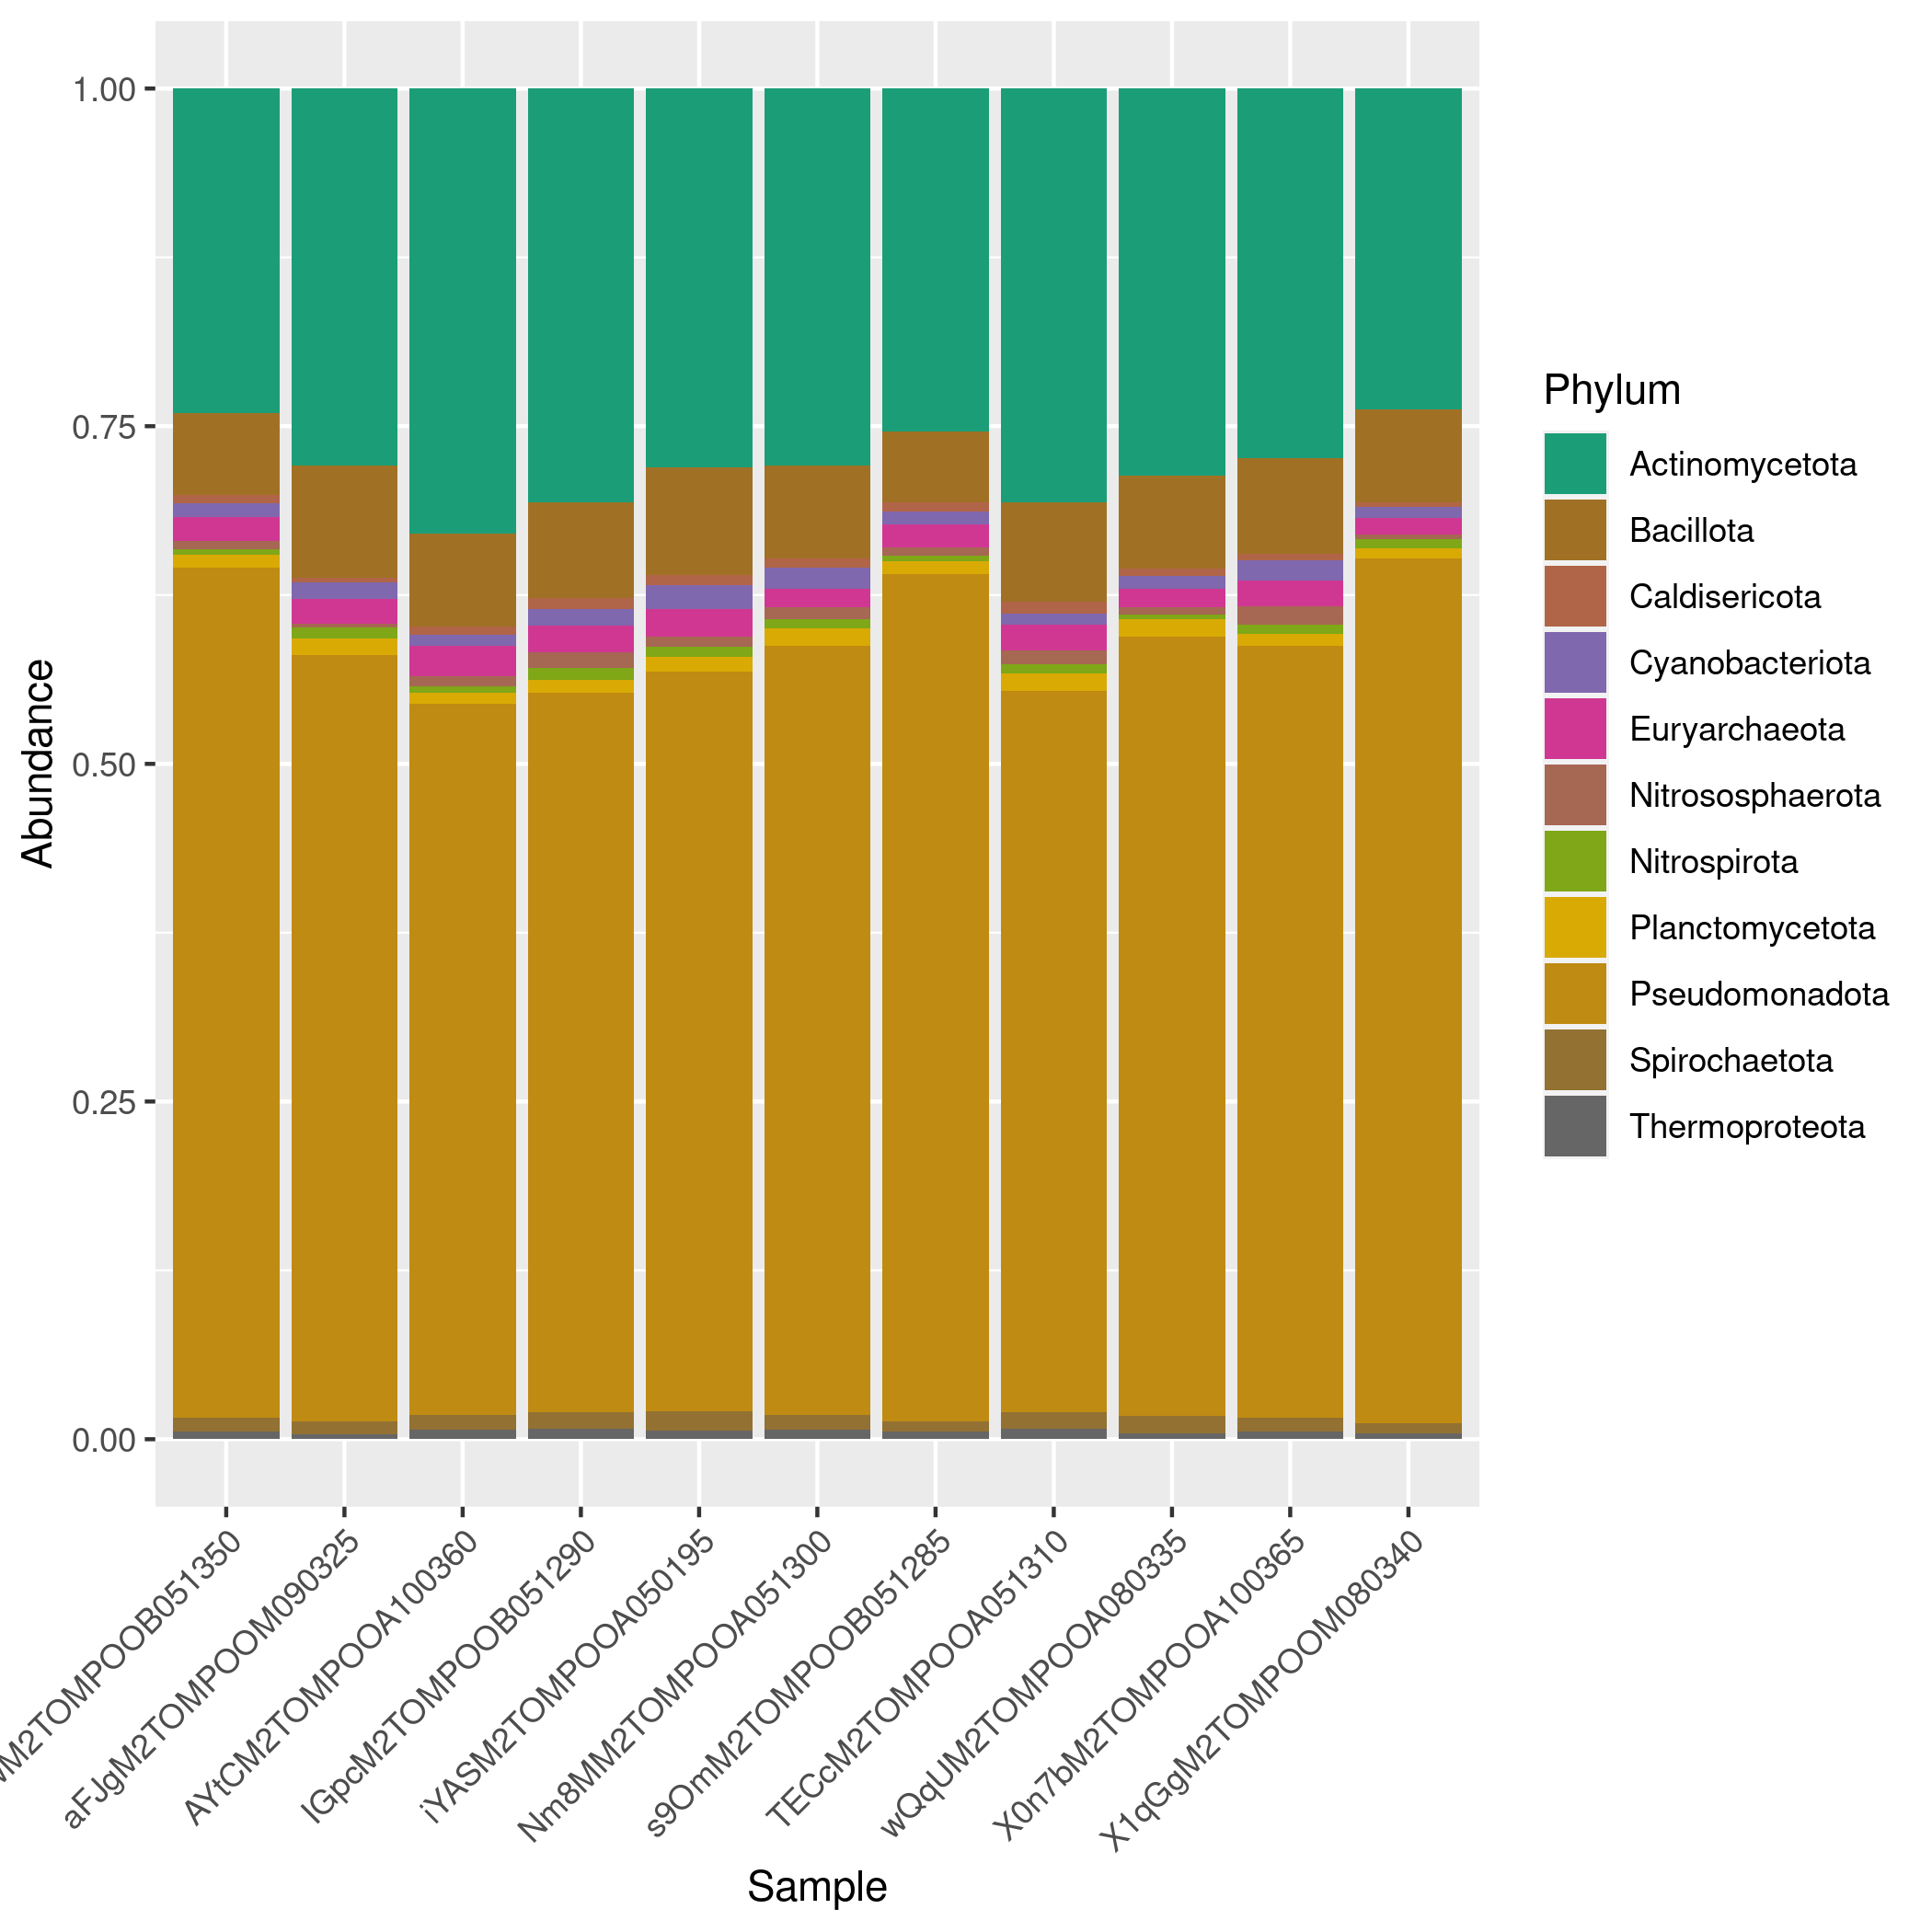
\includegraphics[scale = 0.8]{tomate_aleatorio1_10.csv_relative_abundance_Phylum.png}
\caption{Relative abundance by phyla of keystone OTUs }
\label{fig:tomate_aleatorio1_10.csv_phyla}
\end{figure}
\begin{figure}
\centering
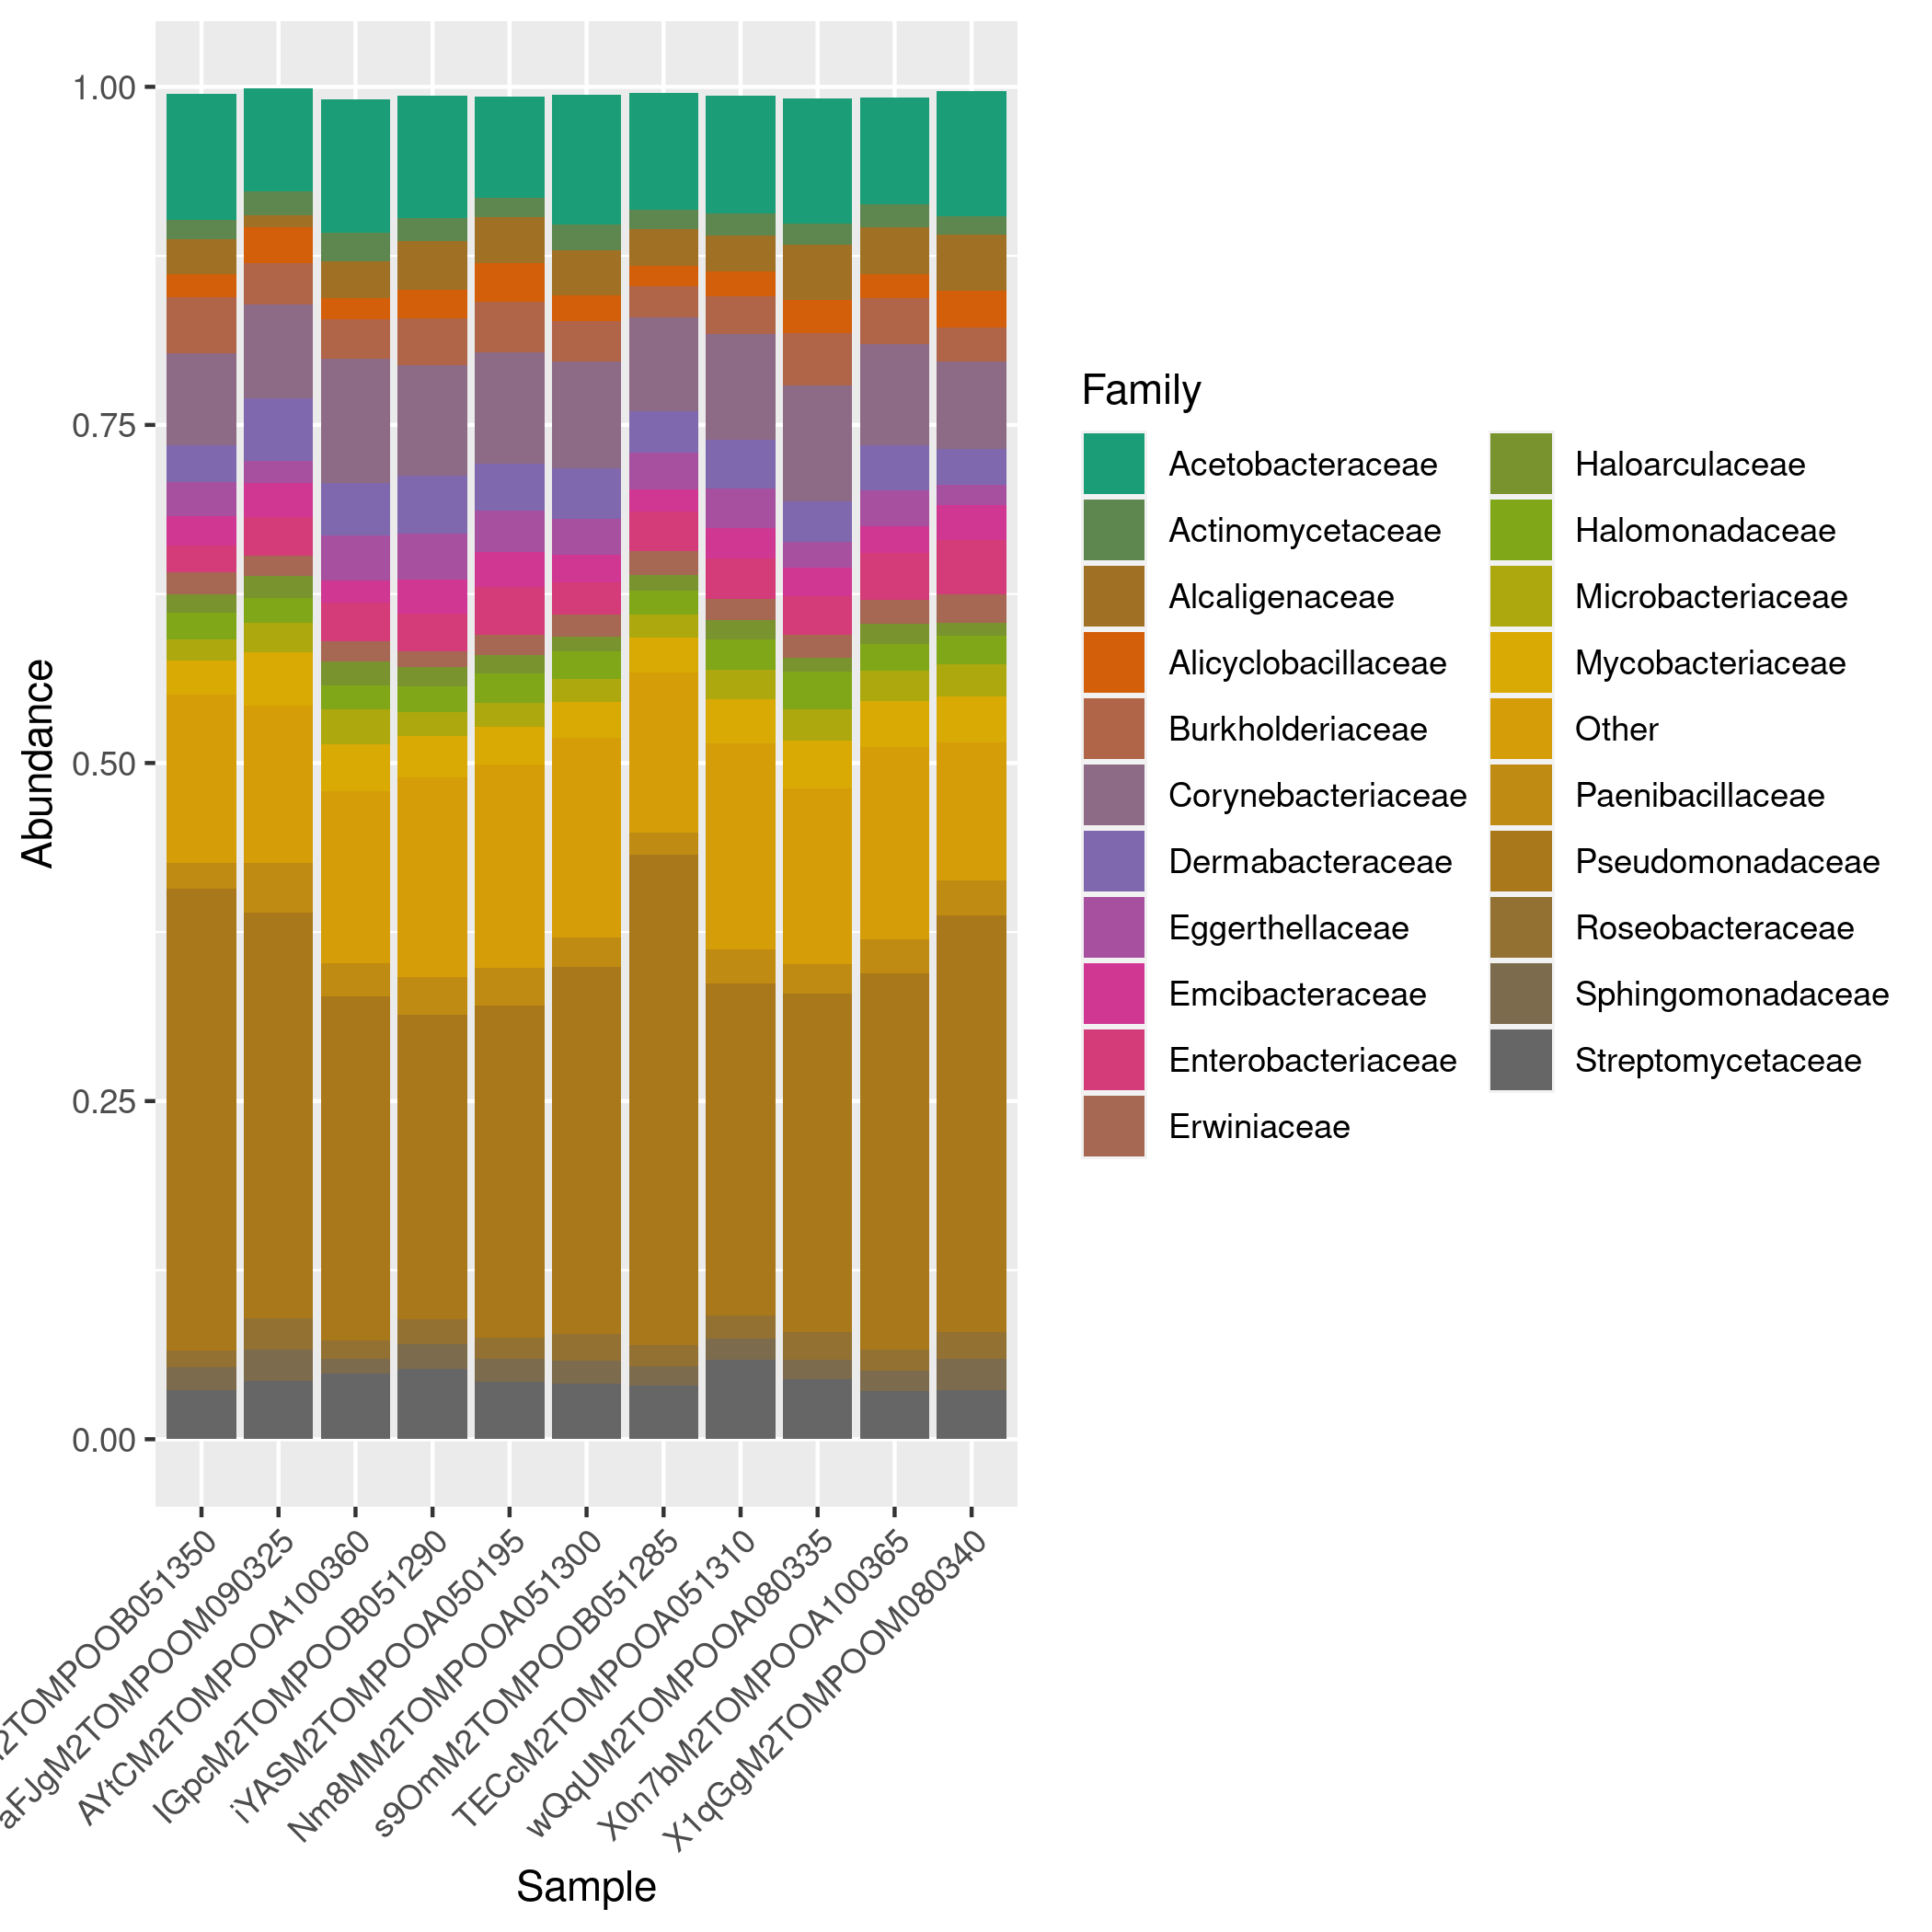
\includegraphics[scale = 0.8]{tomate_aleatorio1_10.csv_relative_abundance_Family.png}
\caption{Relative abundance by families of keystone OTUs }
\label{fig:tomate_aleatorio1_10.csv_family}
\end{figure}
\begin{figure}
\centering
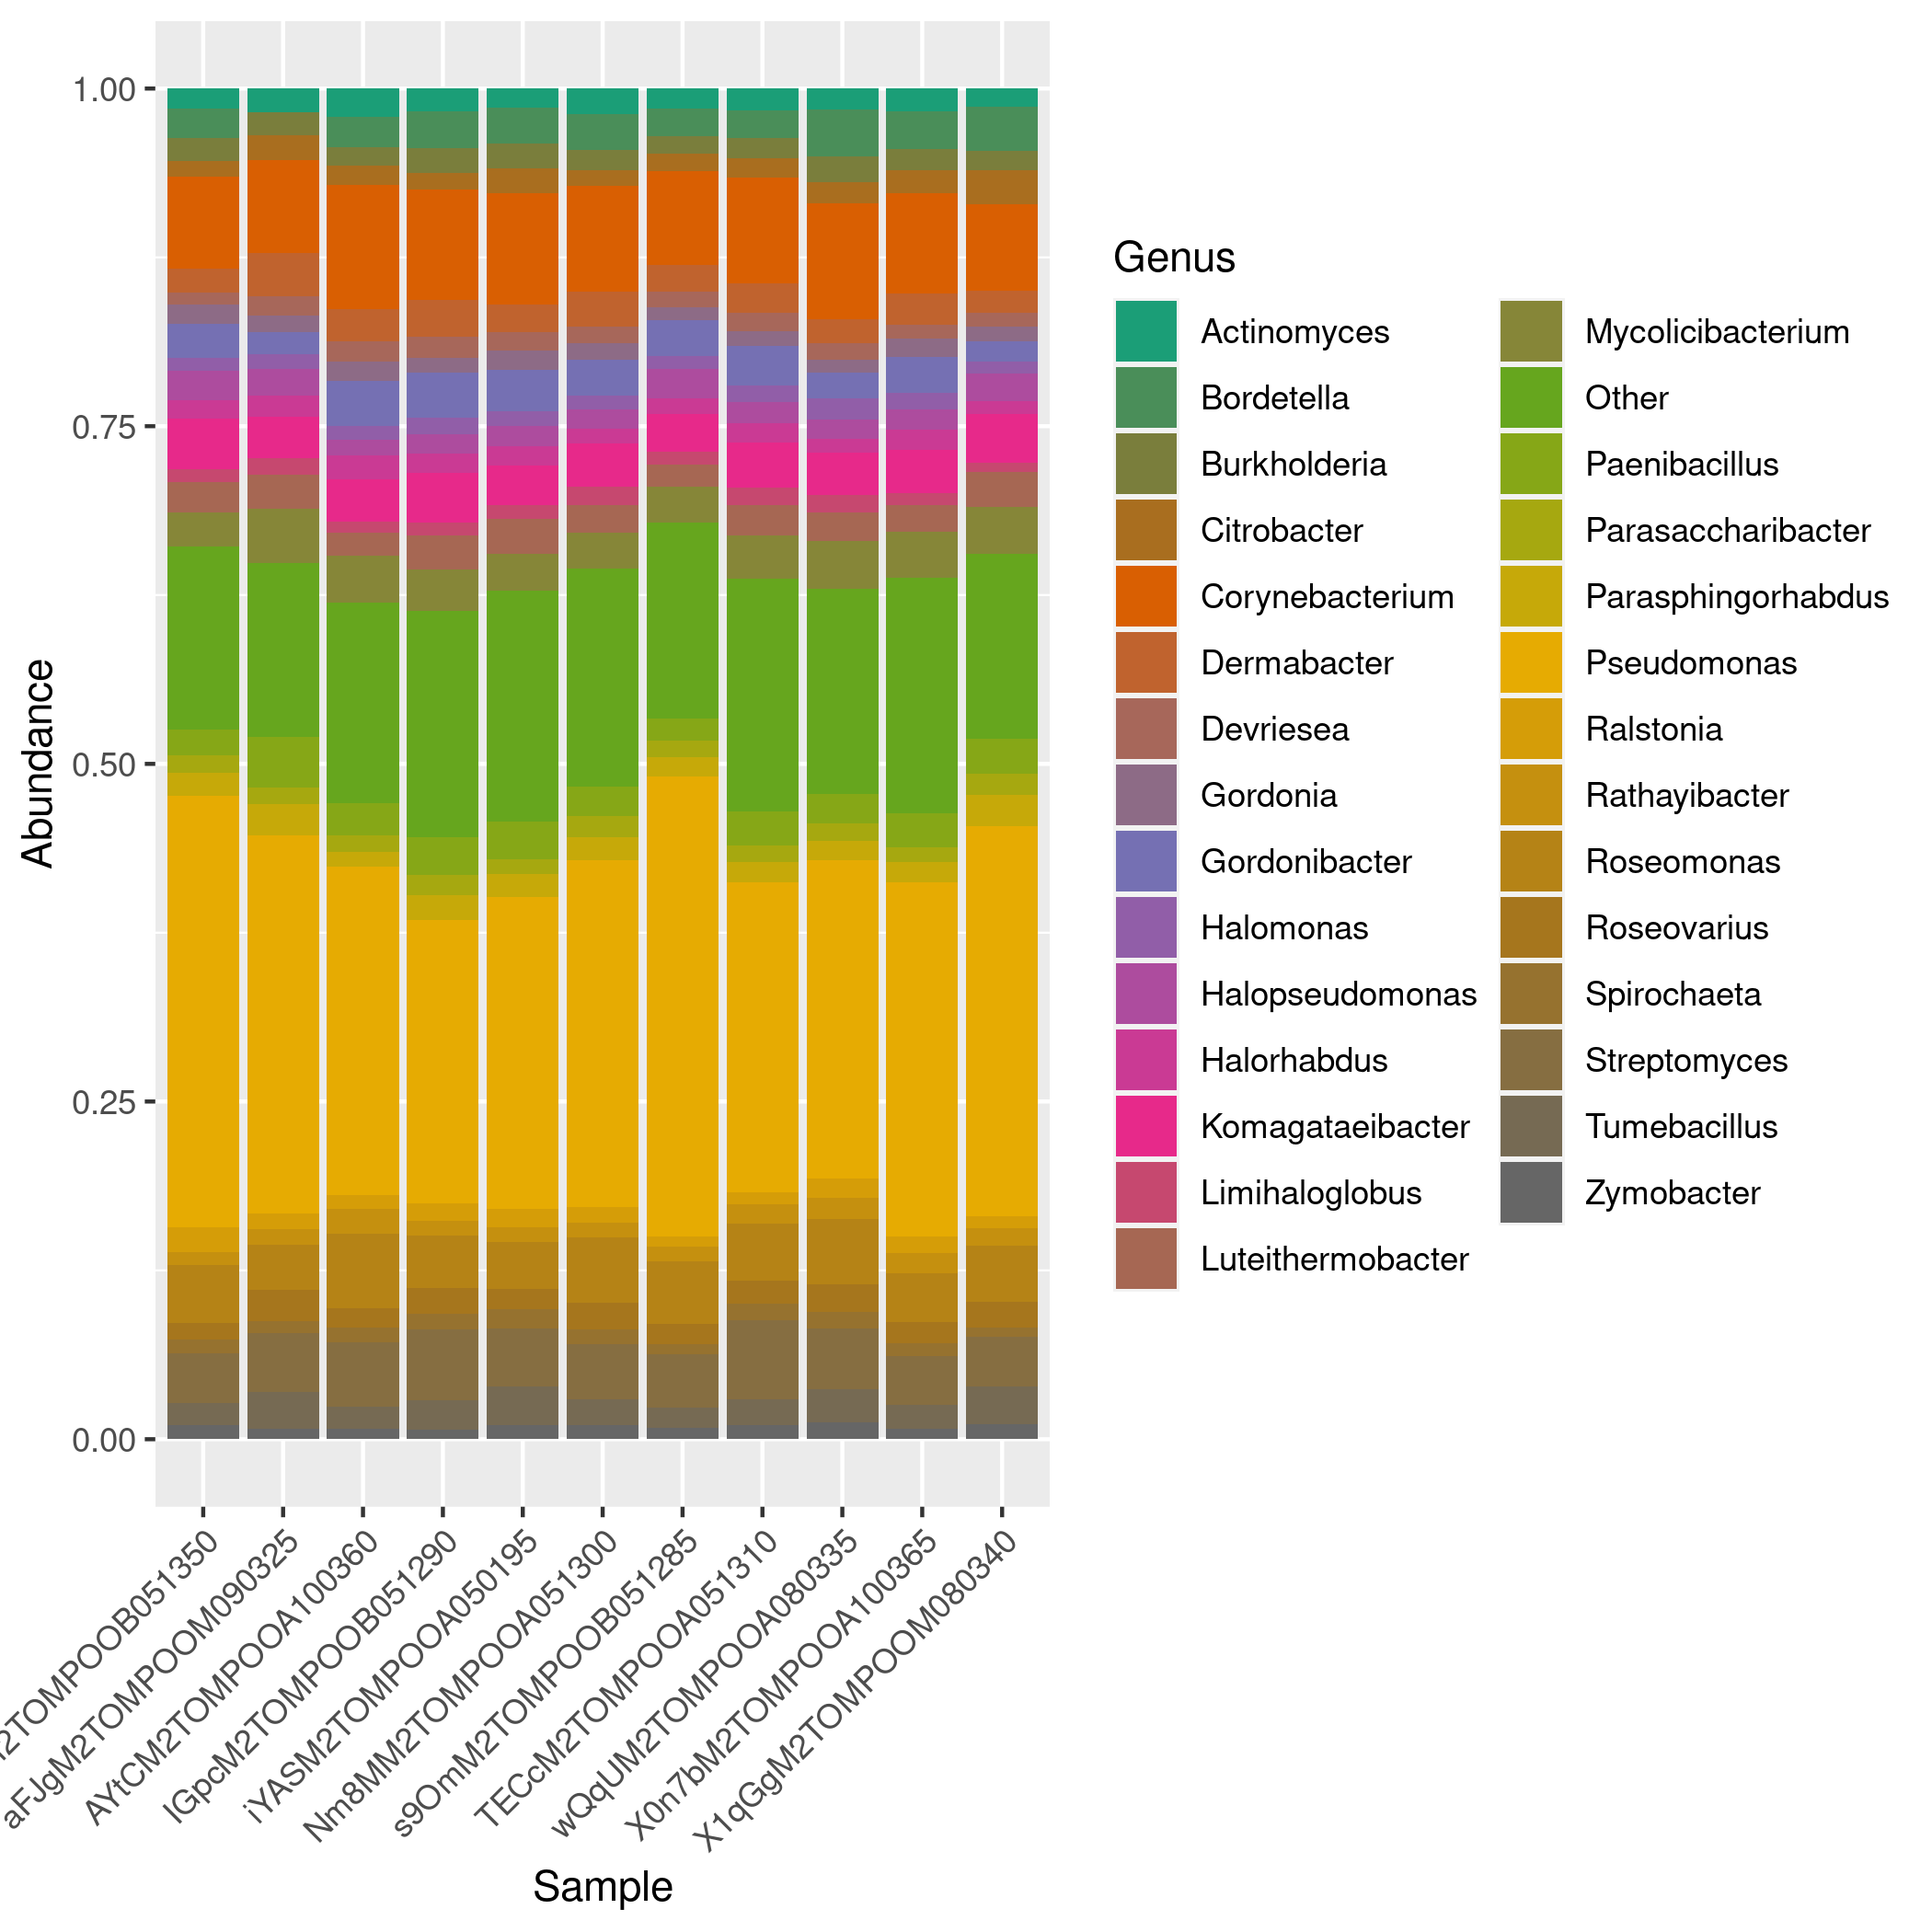
\includegraphics[scale = 0.8]{tomate_aleatorio1_10.csv_relative_abundance_Genus.png}
\caption{Relative abundance by genera of keystone OTUs }
\label{fig:tomate_aleatorio1_10.csv_genus}
\end{figure}
\begin{figure}
   \centering
   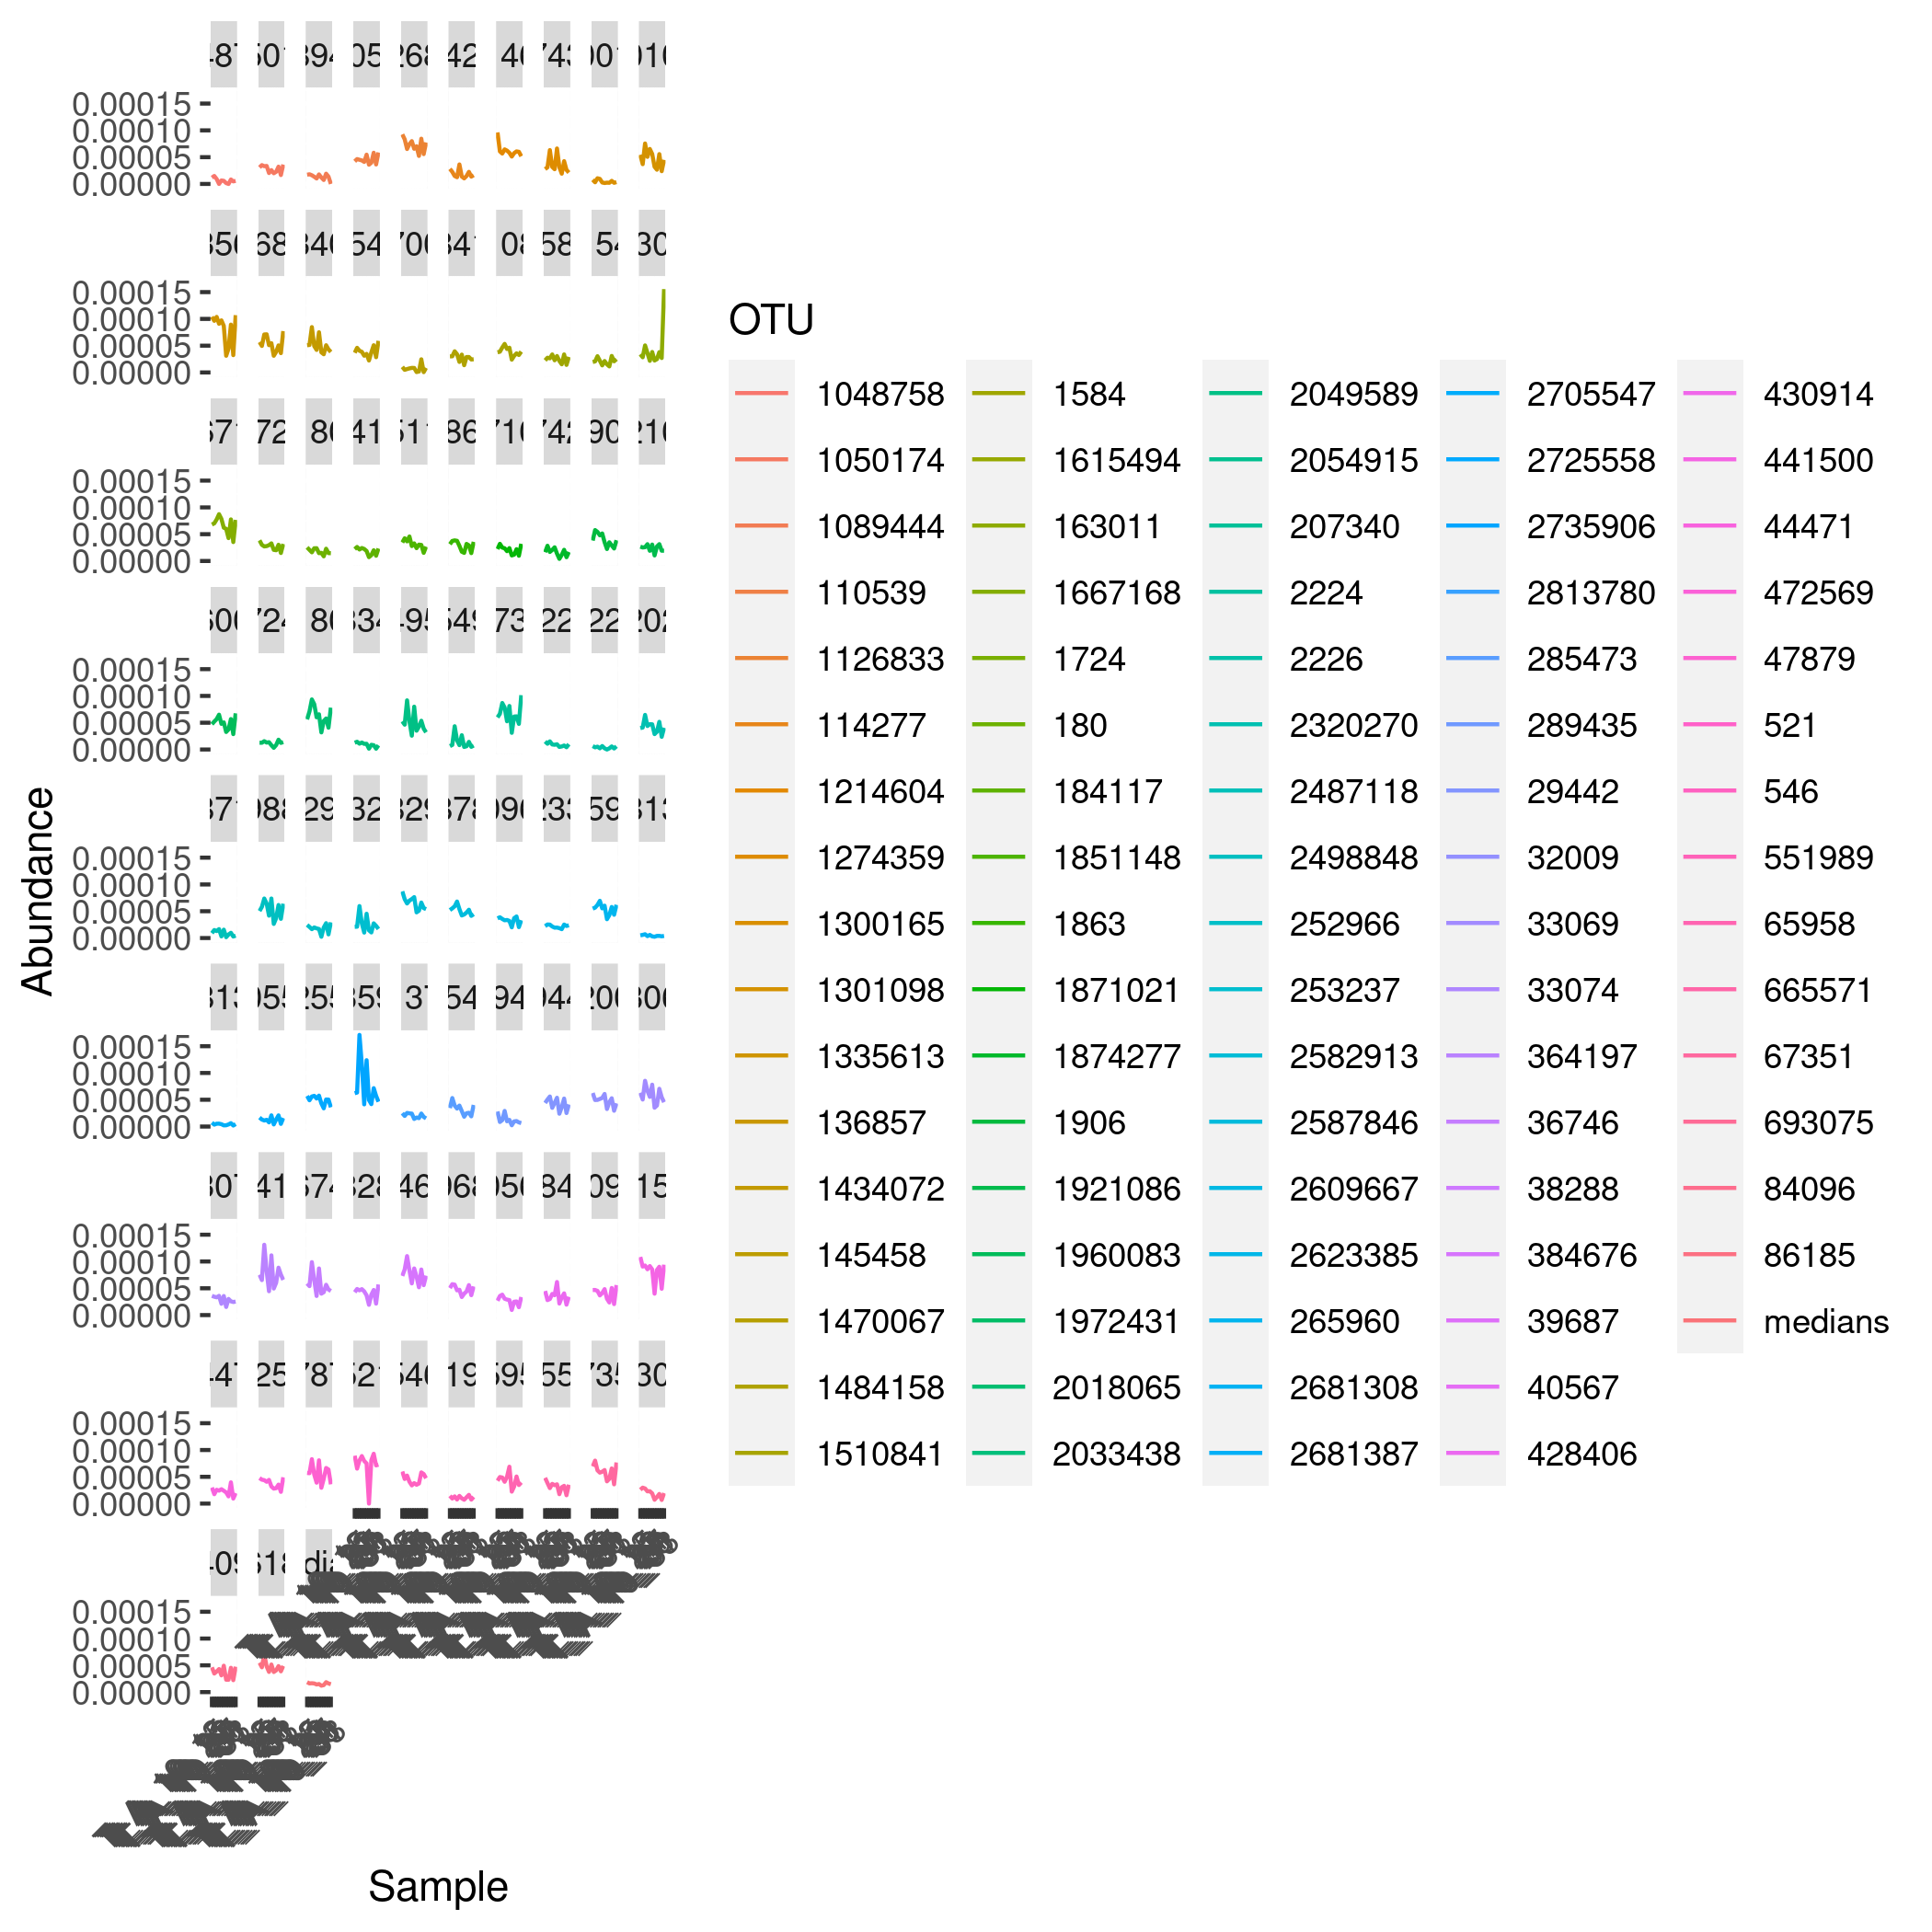
\includegraphics[scale = 0.8]{abundance_tomate_aleatorio1_10.csv_key_otus_medians.png}
   \caption{Plots representing relative abundance of each keystone OTU and one representing the median relative abundance  across samples of rhizosphere of tomate_aleatorio1_10.csv. Most keystone OTUs have relative abundance bigger than the median across all samples.  }
   \label{key_otus_vs_medians_tomate_aleatorio1_10.csv}
\end{figure}
\begin{figure}
 \centering
 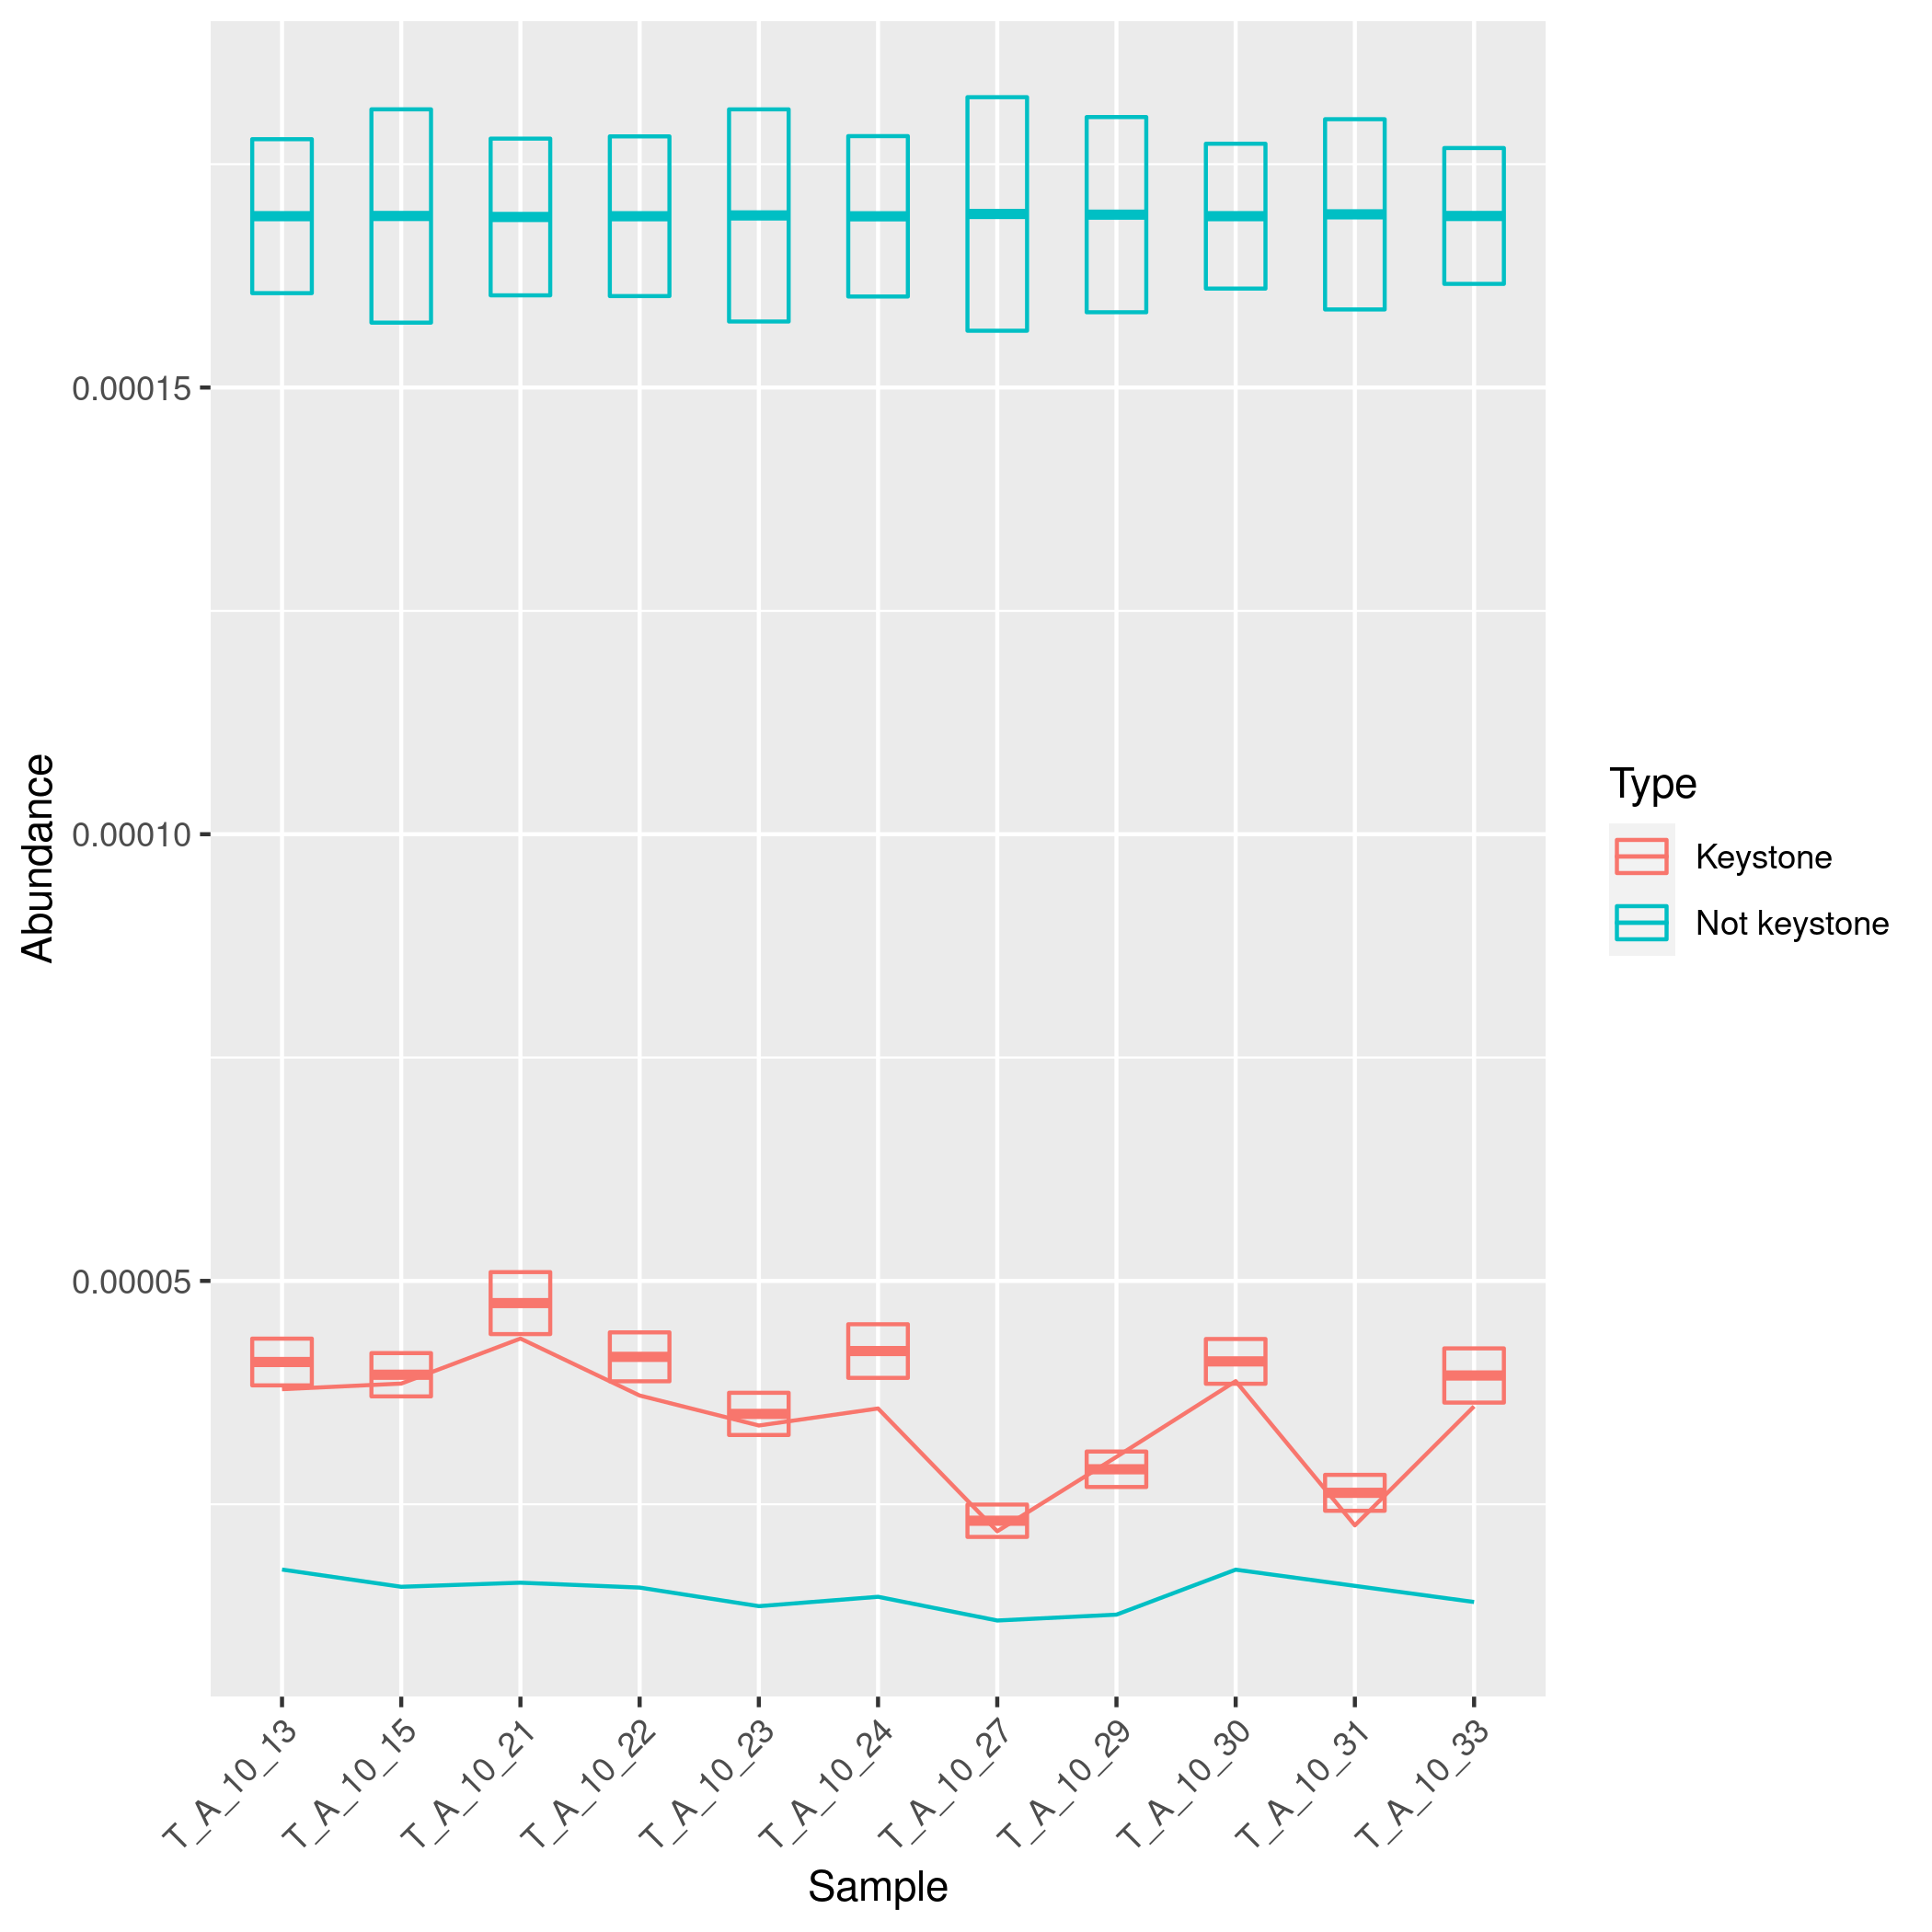
\includegraphics[scale = 0.75]{mean_median_key_vs_not_key_tomate_aleatorio1_10.csv.png}
\caption{Boxes represent mean and standard error in the distribution of corresponding samples. Lines represent the corresponding medians. In these samples of rhizosphere oftomate_aleatorio1_10.csv}
\label{mean_median_tomate_aleatorio1_10.csv}
\end{figure}
\begin{figure}
   \centering
   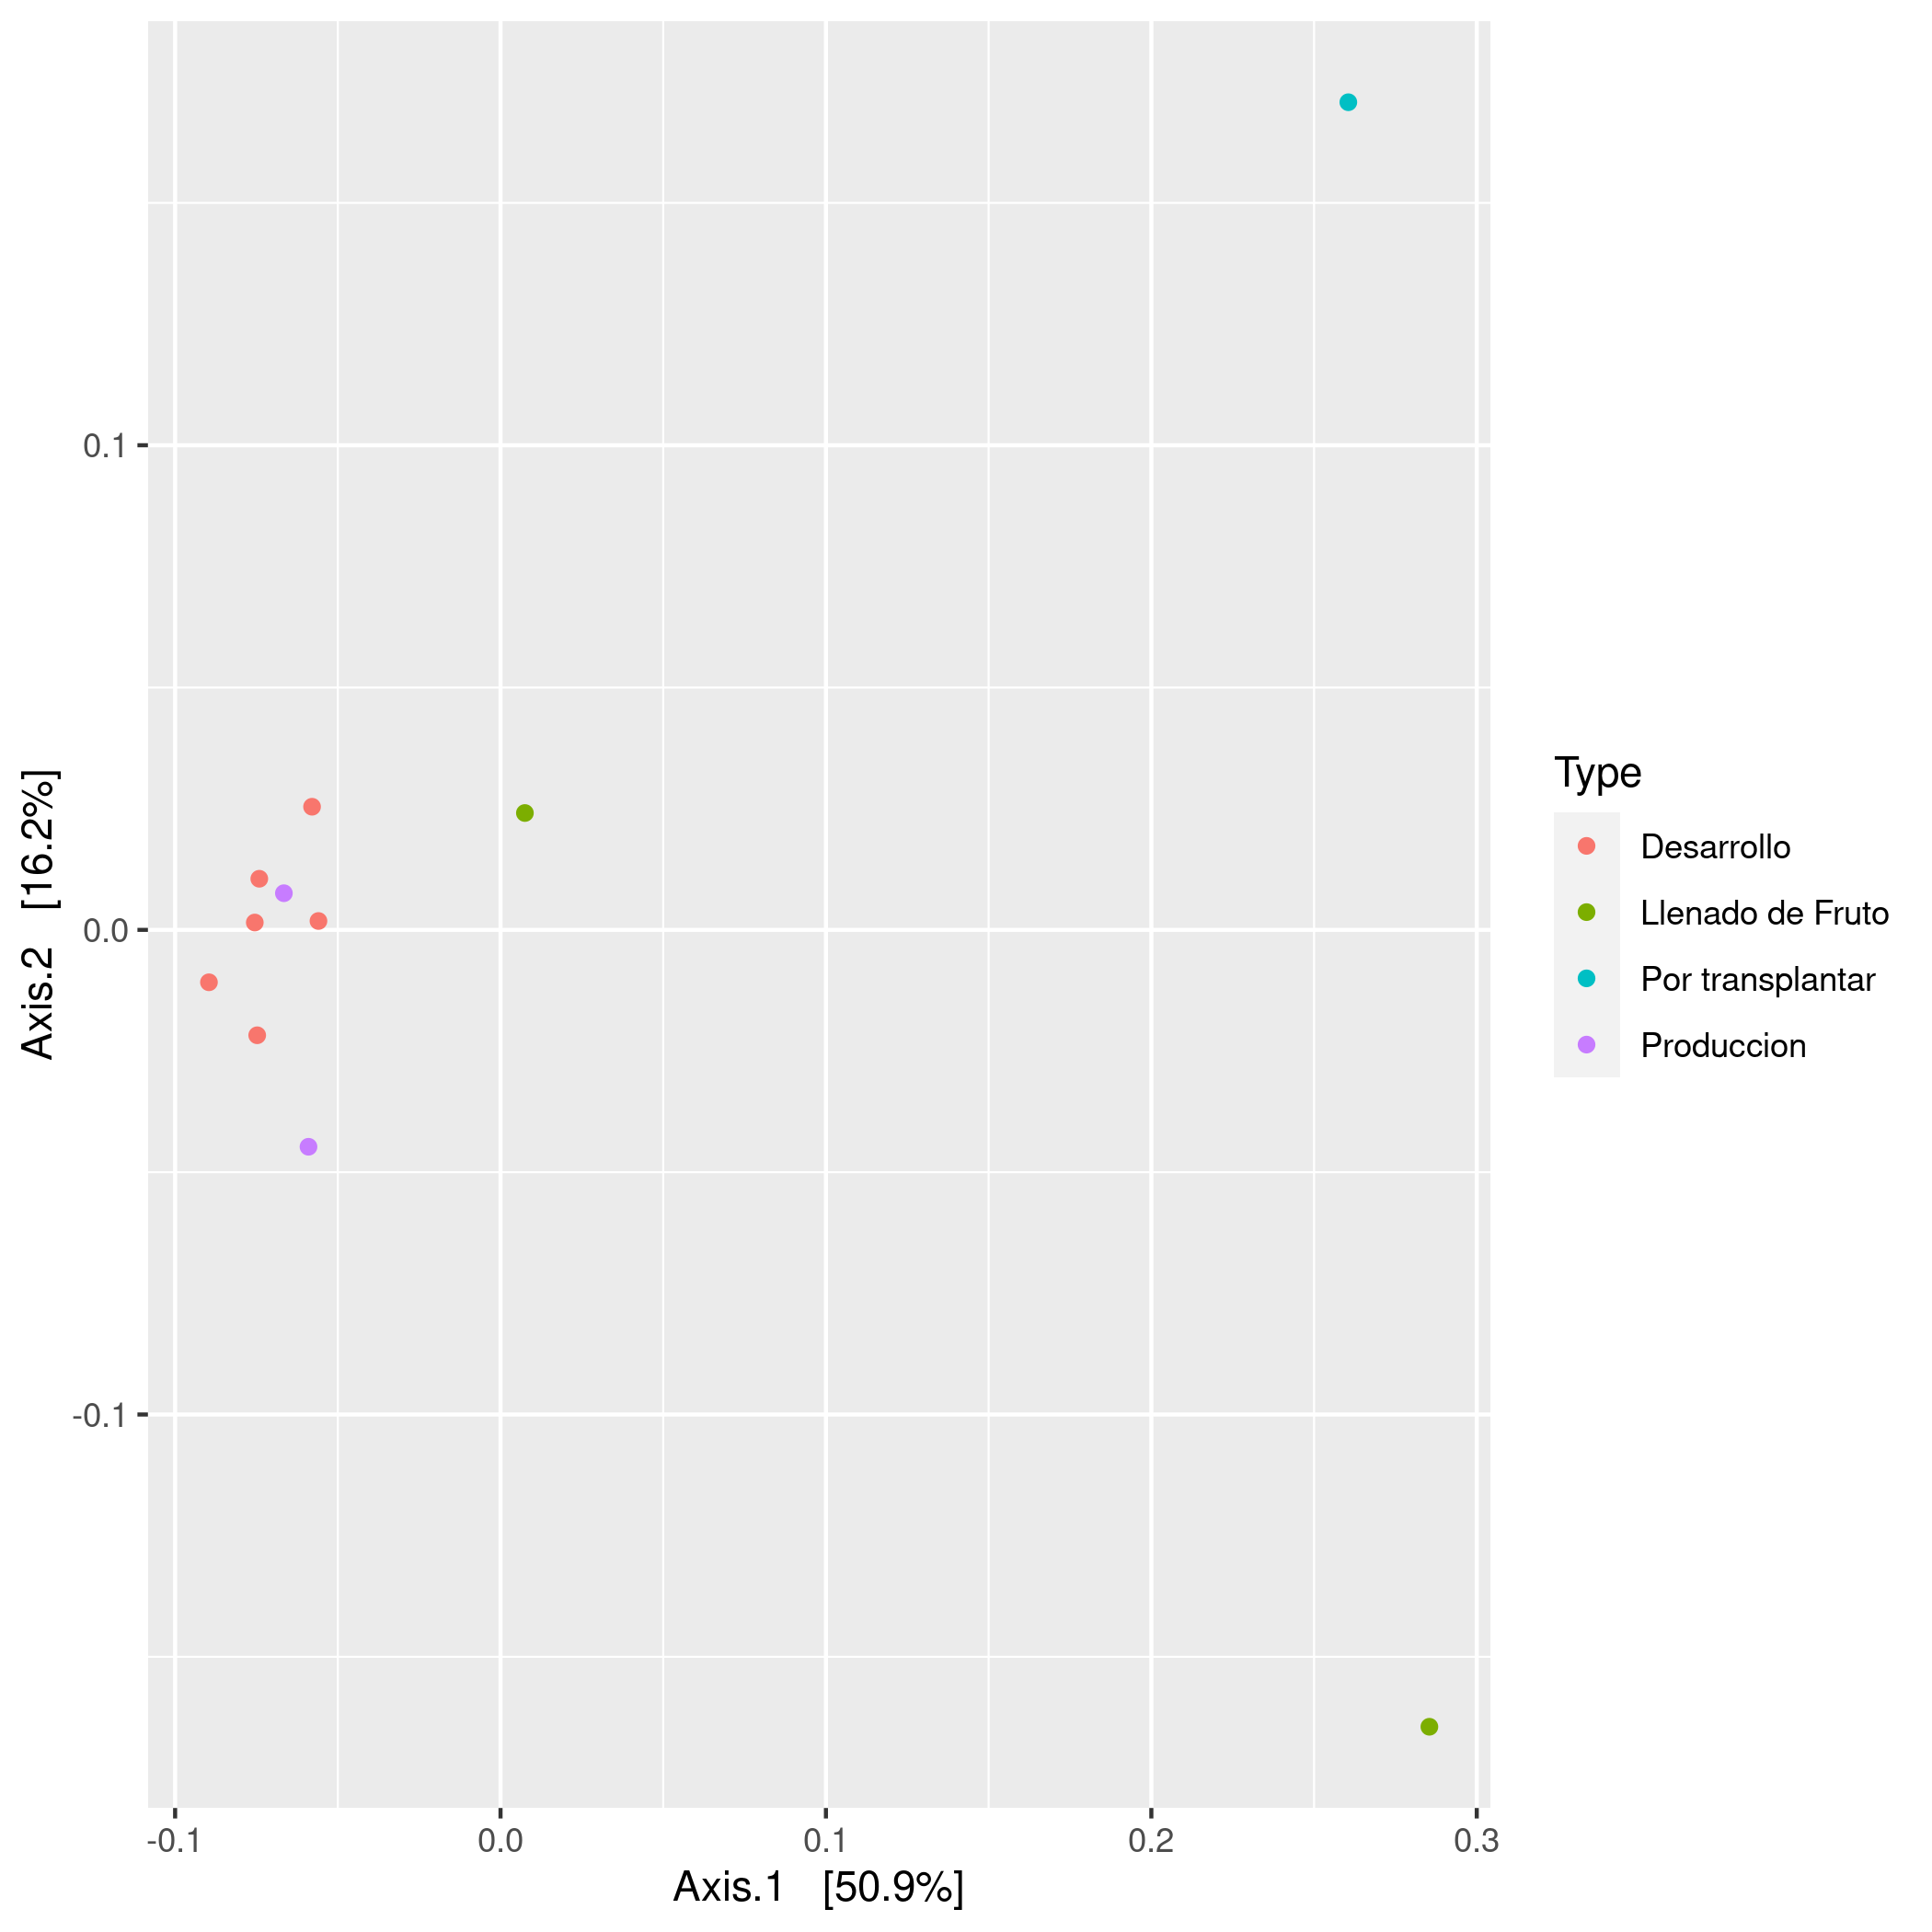
\includegraphics[scale = 0.7]{pcoa_muestras_tomate_aleatorio1_10.csv.png}
 \caption{PCoA analysis with Bray-Curtis distance of rhizosphere samples of tomate_aleatorio1_10.csv.}
 \label{fig:tomate_aleatorio1_10.csv_pcoa}
\end{figure}
\begin{figure}
  \centering
  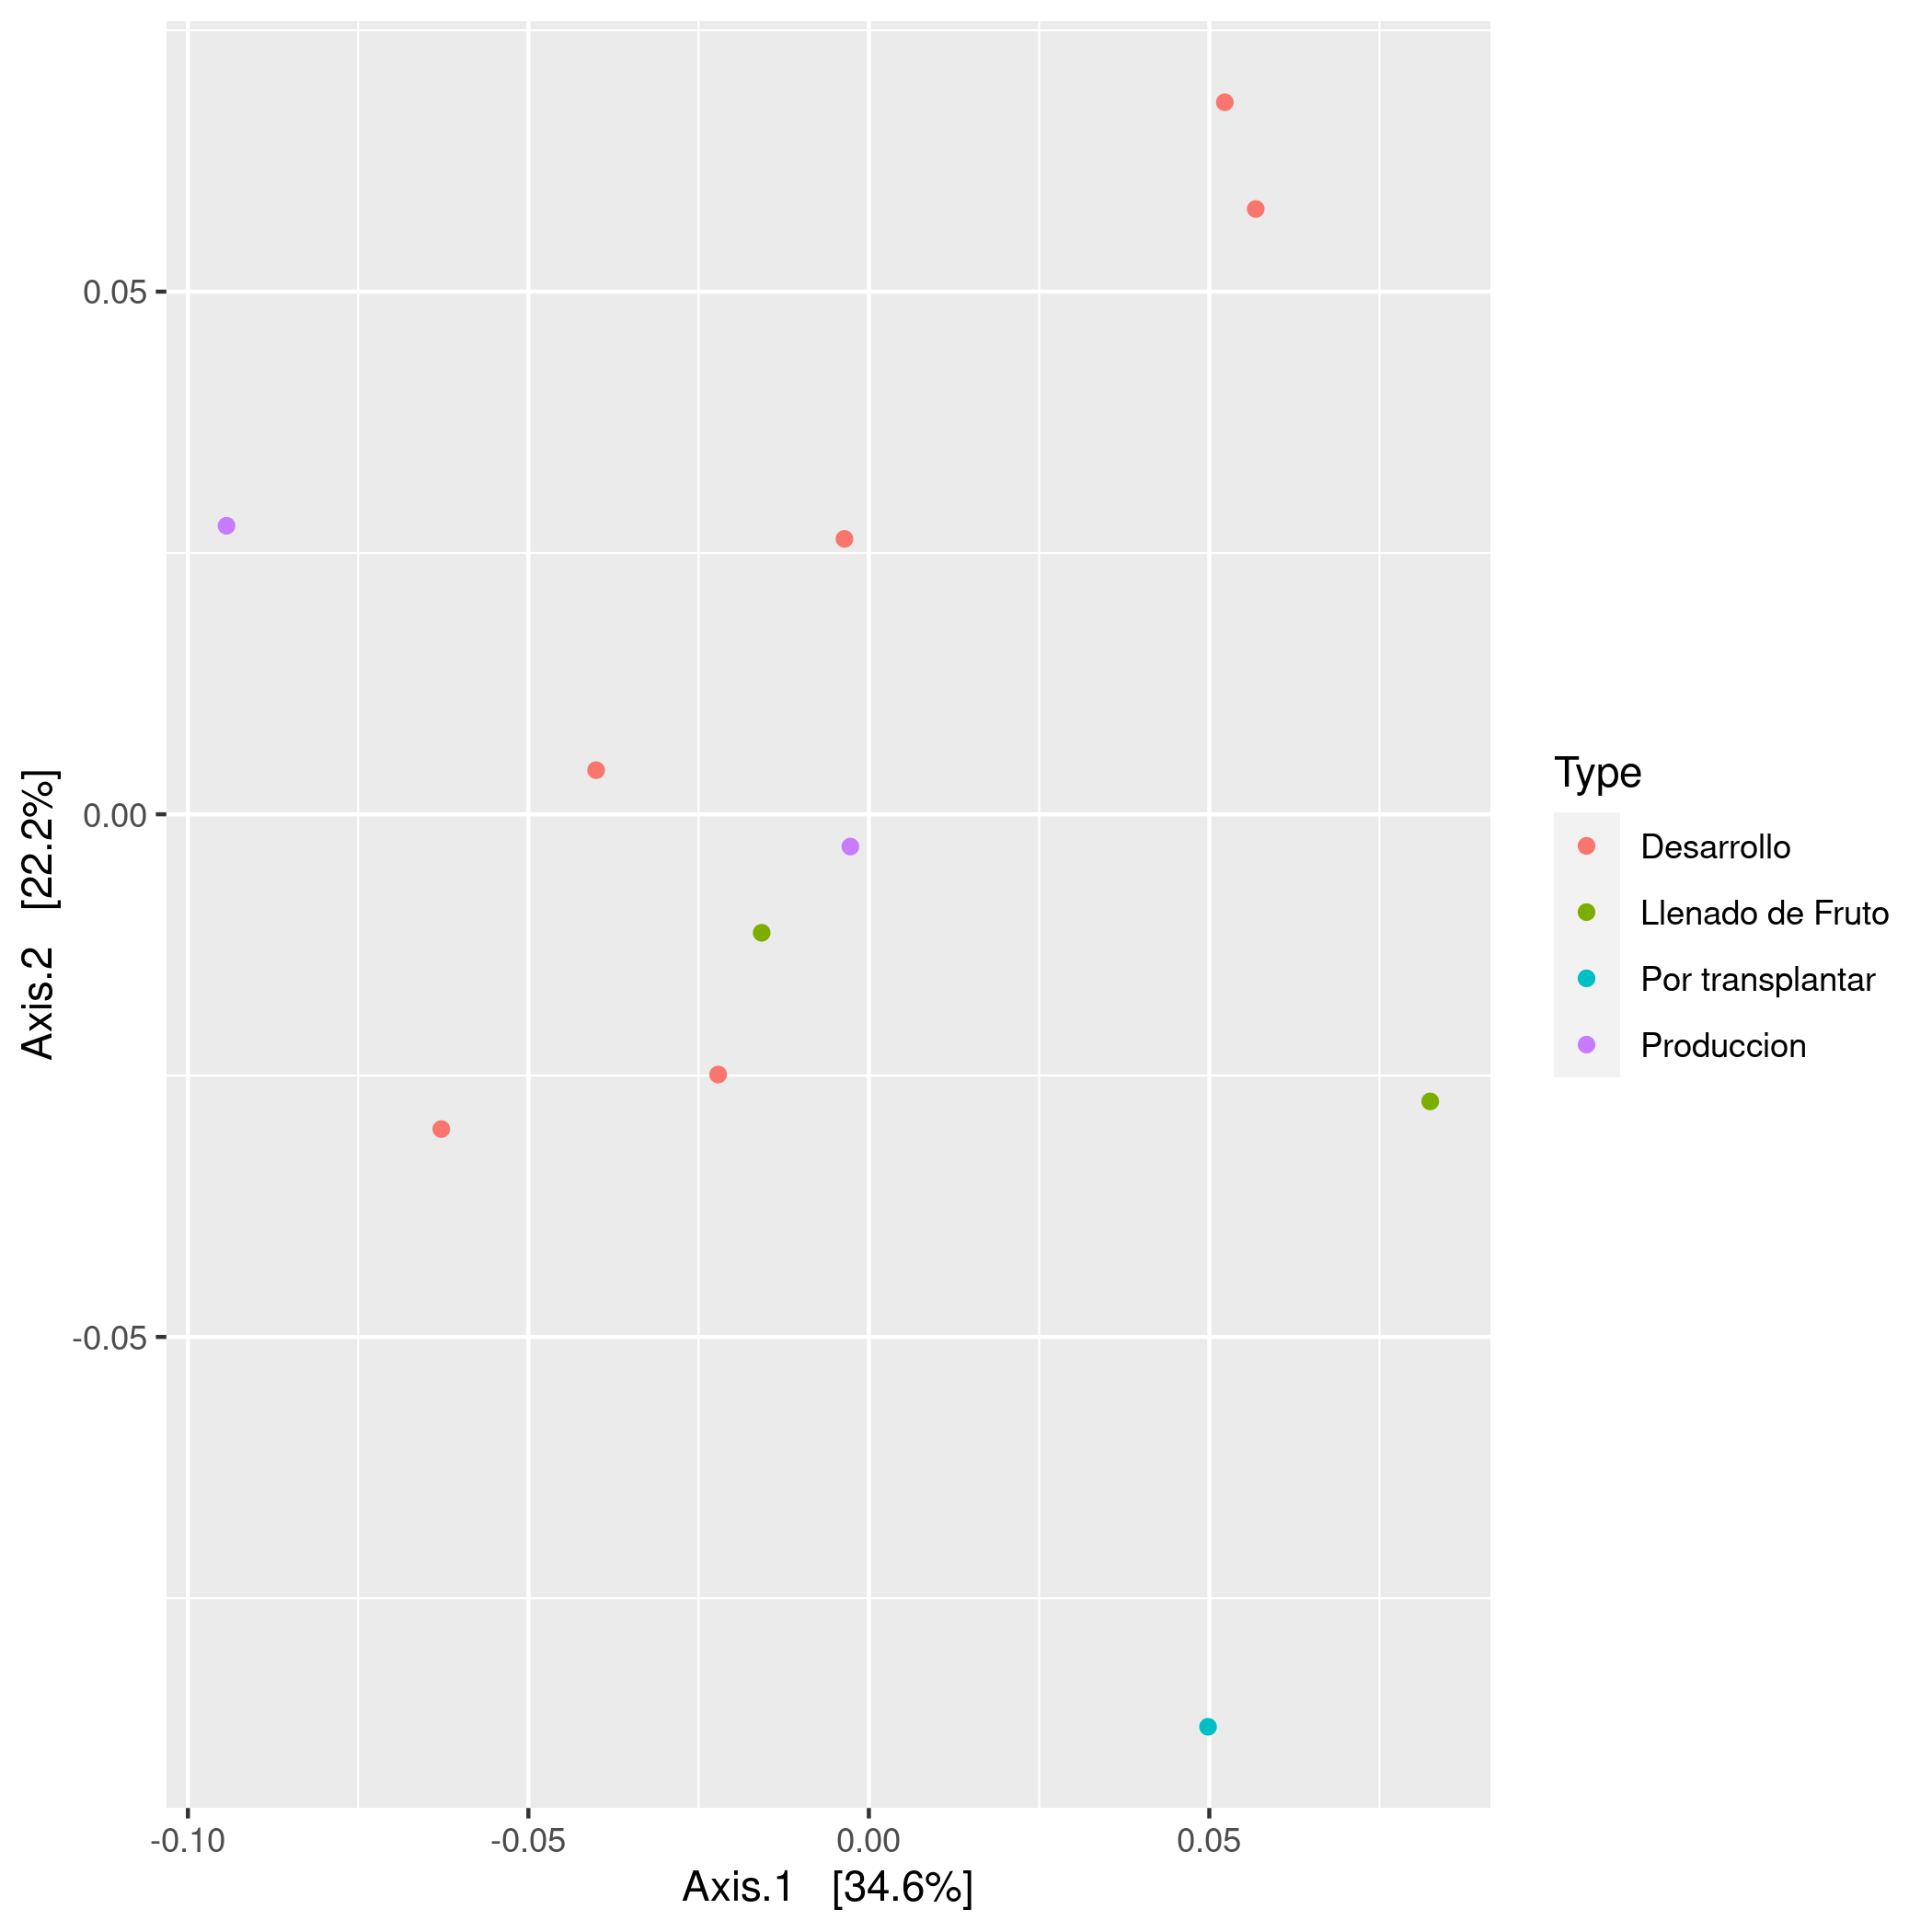
\includegraphics[scale = 0.7]{pcoa_key_otus_tomate_aleatorio1_10.csv.png}
  \caption{PCoA analysis with Bray-Curtis distance of rhizosphere samples of tomate_aleatorio1_10.csv, restricted to keystone OTUs.}
  \label{fig:tomate_aleatorio1_10.csv_pcoa_key_otus}
\end{figure}
